\documentclass[11pt,a4paper]{article}

% ============================================================================
% PACKAGES & TYPOGRAPHY
% ============================================================================
\usepackage[a4paper, top=24mm, bottom=24mm, left=22mm, right=22mm]{geometry}
\usepackage[utf8]{inputenc}
\usepackage[T1]{fontenc}
\usepackage{lmodern}
\usepackage{microtype}
\usepackage{amsmath, amssymb}
\usepackage{graphicx}
\usepackage{booktabs}
\usepackage{tabularx}
\usepackage{multirow}
\usepackage{array}
\usepackage{float}
\usepackage{caption}
\usepackage{subcaption}
\usepackage{enumitem}
\usepackage[dvipsnames,table]{xcolor}
\usepackage{tikz}
\usetikzlibrary{arrows.meta, positioning, shapes.geometric, fit, backgrounds, calc}
\usepackage{tcolorbox}
\tcbuselibrary{skins, breakable}
\usepackage{fancyhdr}
\usepackage{titlesec}
\usepackage{listings}
\usepackage{hyperref}

% ============================================================================
% COLOR PALETTE (ACADEMIC NAVY / TEAL / SLATE)
% ============================================================================
\definecolor{NavyPrimary}{HTML}{0F294A}
\definecolor{RoyalAccent}{HTML}{1D4ED8}
\definecolor{TealAccent}{HTML}{0F766E}
\definecolor{SlateDark}{HTML}{1E293B}
\definecolor{SlateMuted}{HTML}{64748B}
\definecolor{LightBg}{HTML}{F8FAFC}
\definecolor{CardBg}{HTML}{F1F5F9}
\definecolor{AmberBg}{HTML}{FEF3C7}
\definecolor{AmberBorder}{HTML}{D97706}
\definecolor{GreenBg}{HTML}{ECFDF5}
\definecolor{GreenBorder}{HTML}{059669}
\definecolor{BorderGray}{HTML}{CBD5E1}

% ============================================================================
% HYPERREF & SECTION STYLING
% ============================================================================
\hypersetup{
    colorlinks=true,
    linkcolor=NavyPrimary,
    citecolor=TealAccent,
    urlcolor=RoyalAccent,
    pdftitle={FreshGuard: Dynamic Food Clearing House Simulator — Project Report},
    pdfauthor={AIT-201 Applied Machine Learning Team}
}

\titleformat{\section}
    {\Large\bfseries\color{NavyPrimary}}
    {\thesection}{0.8em}{}
    [\vspace{2pt}{\color{RoyalAccent}\titlerule[0.9pt]}]

\titleformat{\subsection}
    {\large\bfseries\color{RoyalAccent}}
    {\thesubsection}{0.7em}{}

\titleformat{\subsubsection}
    {\normalsize\bfseries\color{SlateDark}}
    {\thesubsubsection}{0.6em}{}

\captionsetup{
    font=small,
    labelfont={bf,color=NavyPrimary},
    skip=6pt
}

% ============================================================================
% HEADERS & FOOTERS
% ============================================================================
\pagestyle{fancy}
\fancyhf{}
\fancyhead[L]{\footnotesize\bfseries\color{NavyPrimary}FRESHGUARD --- DYNAMIC FOOD CLEARING HOUSE}
\fancyhead[R]{\footnotesize\color{SlateMuted}AIT-201 Applied Machine Learning Project Report}
\fancyfoot[L]{\footnotesize\color{SlateMuted}Department of Computer Science / Applied ML (Sem 4)}
\fancyfoot[R]{\footnotesize\bfseries\color{SlateDark}Page \thepage}
\renewcommand{\headrulewidth}{0.5pt}
\renewcommand{\footrulewidth}{0.5pt}
\renewcommand{\headrule}{\hbox to\headwidth{\color{BorderGray}\leaders\hrule height \headrulewidth\hfill}}
\renewcommand{\footrule}{\hbox to\headwidth{\color{BorderGray}\leaders\hrule height \footrulewidth\hfill}}

% ============================================================================
% CALLOUT BOXES & CODE STYLE
% ============================================================================
\newtcolorbox{keyfinding}[1][]{
    enhanced,
    breakable,
    colback=LightBg,
    colframe=NavyPrimary,
    boxrule=0.6pt,
    leftrule=3.5pt,
    arc=2pt,
    top=6pt, bottom=6pt, left=8pt, right=8pt,
    fonttitle=\bfseries\small\color{NavyPrimary},
    title=#1
}

\newtcolorbox{auditnote}[1][]{
    enhanced,
    breakable,
    colback=AmberBg,
    colframe=AmberBorder,
    boxrule=0.6pt,
    leftrule=3.5pt,
    arc=2pt,
    top=6pt, bottom=6pt, left=8pt, right=8pt,
    fonttitle=\bfseries\small\color{AmberBorder},
    title=#1
}

\lstset{
    basicstyle=\ttfamily\scriptsize\color{SlateDark},
    backgroundcolor=\color{CardBg},
    frame=single,
    rulecolor=\color{BorderGray},
    breaklines=true,
    captionpos=b,
    xleftmargin=4pt,
    xrightmargin=4pt,
    aboveskip=6pt,
    belowskip=6pt
}

\setlength{\parskip}{4pt}
\setlength{\parindent}{0pt}

% ============================================================================
% BEGIN DOCUMENT
% ============================================================================
\begin{document}

% ----------------------------------------------------------------------------
% TITLE PAGE
% ----------------------------------------------------------------------------
\begin{titlepage}
    \thispagestyle{empty}
    \vspace*{6mm}
    {\color{RoyalAccent}\rule{\textwidth}{2.5pt}}
    \vspace{6mm}

    {\small\bfseries\color{TealAccent}\uppercase{AIT-201 Applied Machine Learning \textbullet\ Final Technical Project Report}}

    \vspace{5mm}
    {\Huge\bfseries\color{NavyPrimary}FreshGuard: Dynamic Food Clearing House Simulator\par}
    \vspace{3.5mm}
    {\Large\color{SlateDark}Proactive Retail Food Waste Prevention via Machine Learning Spoilage Prediction, Multi-Horizon Demand Forecasting, Anti-Moral-Hazard Clearance Policy, and Smart OSRM Logistics\par}

    \vspace{6mm}
    {\color{BorderGray}\rule{\textwidth}{0.8pt}}
    \vspace{6mm}

    \begin{tcolorbox}[
        colback=LightBg,
        colframe=BorderGray,
        boxrule=0.7pt,
        arc=3pt,
        top=10pt, bottom=10pt, left=12pt, right=12pt
    ]
        \renewcommand{\arraystretch}{1.28}
        \begin{tabularx}{\textwidth}{@{} >{\bfseries\color{NavyPrimary}}l X @{}}
            Course:          & AIT-201 Applied Machine Learning (Year 2, Semester 4) \\
            System Name:     & FreshGuard --- Dynamic Food Clearing House (Malaysia Retail Scope) \\
            Architecture:    & Two-Phase Modular Pipeline (Phase 1 BASE + Phase 2 UPGRADE) \\
            Core Stack:      & Python (XGBoost, LightGBM, Scikit-Learn), FastAPI, Supabase PostgreSQL, React 18 + Vite, OSRM Routing \\
            Localization:    & Malaysian Ringgit (MYR), OpenDOSM PriceCatcher, 2025--2026 Malaysian Holidays, Klang Valley Food Banks \\
            Report Date:     & November 18, 2026 \\
        \end{tabularx}
    \end{tcolorbox}

    \vspace{7mm}
    {\normalsize\bfseries\color{NavyPrimary}Project Team \& Engineering Role Matrix}\\[4pt]
    \renewcommand{\arraystretch}{1.22}
    {\footnotesize
    \begin{tabularx}{\textwidth}{@{} c >{\bfseries}l l X @{}}
        \toprule
        \rowcolor{NavyPrimary}
        \color{white}\textbf{Role} & \color{white}\textbf{Title} & \color{white}\textbf{Assigned Goals} & \color{white}\textbf{Primary Shipped Deliverables} \\
        \midrule
        Person 0 & Dataset Quality Specialist & Data Prep \& Audit & 12 cleaned datasets, 496 expiry repairs, SMOTE bootstrap, \texttt{holidays\_my.csv}, DOSM Parquet \\
        \rowcolor{LightBg}
        Person 1 & Tech Lead \& Spoilage ML & Goal 1 (Step 7) & Two-tier XGBoost classifier (\texttt{spoilage\_classifier.pkl}), dual-weighted model, FEFO sorter \\
        Person 2 & Forecaster \& API Engineer & Goals 2 \& 10 (Step 8) & 3-horizon LightGBM models (\texttt{demand\_forecast\_final\_day\_\{1,2,3\}.pkl}), FastAPI REST server \\
        \rowcolor{LightBg}
        Person 3 & Data Architect \& Pipeline & Goals 3 \& 4 (Steps 9--10) & Single-store ETL (\texttt{lots\_base.csv}), 7-rule validator, canonical schema, 2,644-event simulator \\
        Person 4 & Business Logic \& Cloud DB & Goals 6 \& 9 (Step 12) & Anti-moral-hazard rule engine (45/45 tests), Supabase 5-table schema + RLS + live ingestion \\
        \rowcolor{LightBg}
        Person 5 & Risk \& Smart Dispatch Lead & Goals 5 \& 7 (Step 11, 13) & ML cargo estimator ($R^2 = 95.5\%$), vehicle/cold-chain specs, live OSRM Klang Valley routing \\
        Person 6 & Frontend, GIS \& Visual Lead & Goals 11 \& 12 (UI/UX) & React 18 + Vite 6-step store dashboard, POS sales log, SVG charts, pre-rendered route preview \\
        \bottomrule
    \end{tabularx}}

    \vfill
    \begin{center}
        {\footnotesize\color{SlateMuted}Every quantitative metric, confusion matrix entry, feature importance score, and operational KPI in this report is derived directly from executed project scripts and verified artifacts in the repository.}
    \end{center}
\end{titlepage}

% ----------------------------------------------------------------------------
% ABSTRACT
% ----------------------------------------------------------------------------
\begin{abstract}
\noindent Retail grocery supply chains traditionally manage perishable inventory reactively: stock moves on First-In First-Out (FIFO) rules, discounts are improvised at the last minute, and edible surplus is either donated ad-hoc or discarded into landfills. \textbf{FreshGuard} reframes retail food waste from a post-hoc rescue problem into a proactive \emph{Dynamic Food Clearing House} that treats every perishable lot as a depreciating economic asset across Steps 7--14 of the food supply chain.

We design, implement, and evaluate a full-stack Applied Machine Learning platform localized for Malaysian retail operations. The architecture combines five tightly coupled subsystems: (1) a 10-step data preprocessing and canonical ETL pipeline (harmonizing 12 raw tables into 990 validated store lots and a 2,644-event retail lifecycle ledger); (2) a non-circular, zero-leakage two-tier \textbf{XGBoost Spoilage Risk Classifier} trained on 89,880 perishable receipts (achieving \textbf{67.33\% accuracy} and \textbf{0.5127 macro-F1}, outperforming the standard retail Days-To-Expiry heuristic by \textbf{+35.07 percentage points} in accuracy and \textbf{+24.29 pp} in macro-F1, while Tier-2 exponential time-decay escalation lifts HIGH-risk recall to \textbf{71.46\%} at $\alpha=0.10$); (3) three direct multi-horizon \textbf{LightGBM Demand Forecasters} trained on 1.27 million M5 food-retail records (achieving \textbf{12.48\% / 12.84\% / 13.22\% WAPE} across Days +1 to +3, reducing error by \textbf{17.4\%--22.0\%} relative to a strong 7-day seasonal-naive benchmark); (4) an auditable \textbf{Dynamic Markdown \& Anti-Moral-Hazard Rule Engine} enforcing tiered 15\%--40\% commercial clearance, closed-channel NGO segregation, and a strict 30\% per-store donation cap (protecting \textbf{RM~1,312,200.96} in expected value across 990 lots and achieving an \textbf{87.0\% terminal rescue rate} in simulation); and (5) an \textbf{ML Cargo Estimator} ($R^2 = 95.5\%$) paired with live \textbf{OSRM} driving-route dispatch, \textbf{Supabase PostgreSQL} persistence, \textbf{FastAPI}, and a \textbf{React 18 + Vite} executive dashboard. Crucially, we maintain rigorous scientific governance by auditing temporal and granularity gaps in historical demand data, exposing explicit \texttt{not\_validated} advisory badges in the UI and locking automated Purchase Orders.
\end{abstract}

\vspace{4mm}
\tableofcontents
\listoffigures
\listoftables
\newpage

% ============================================================================
% SECTION 1: INTRODUCTION & PROBLEM STATEMENT
% ============================================================================
\section{Introduction and Problem Statement}

\subsection{Background: Reactive Failure Modes in Grocery Retail}
Global food loss and waste assessments by the Food and Agriculture Organization (FAO)~\cite{fao2019} establish that substantial edible loss occurs during post-harvest distribution and retail operations because inventory systems react \emph{after} biological deterioration has already eroded commercial value. In conventional supermarkets, four structural failures compound retail food waste:
\begin{enumerate}[leftmargin=18pt, itemsep=2pt]
    \item \textbf{Shelf-Life Blindness (FIFO vs.\ FEFO):} Warehouses and store shelves routinely rotate stock by arrival date rather than remaining economic shelf life, causing high-value lots with shorter supplier expiration horizons to spoil behind fresher batches.
    \item \textbf{Static Heuristic Escalation:} Traditional retail rules flag items strictly by a fixed Days-To-Expiry (DTE) cutoff (e.g., $\text{DTE} \le 7$), ignoring product sales velocity and stock-to-demand cover. As our empirical evaluation proves (§\ref{sec:spoilage_results}), a pure DTE rule misclassifies 60\% of safe receipts as high-risk, triggering unnecessary margin erosion.
    \item \textbf{Consumer Moral Hazard and Revenue Cannibalization:} Unstructured free giveaways or predictable end-of-day shelf donations incentivize \emph{strategic waiting}, where price-sensitive shoppers withhold full-price purchases to wait for free or heavily discounted food.
    \item \textbf{Fragmented Data and Unmeasured Logistics:} Inventory logs, point-of-sale (POS) sales, commodity reference prices, and charitable food bank capacities reside in disconnected silos, leaving stores unable to verify food rescued, cold-chain vehicle fit, or Environmental, Social, and Governance (ESG) audit trails.
\end{enumerate}

\subsection{Paradigm Shift: Managing Economic Shelf Life}
FreshGuard shifts the operational question from \emph{``How do we rescue food that is already left over?''} to \emph{``At what exact point in its shelf life must a batch transition between commercial sale, tiered dynamic markdown, and closed charitable dispatch to maximize combined economic and social value?''}

We explicitly bound the system to \textbf{Steps 7--14 of the food supply chain} (warehouse FEFO intake, demand-informed allocation, surplus/spoilage detection, clearance channel recommendation, OSRM food-bank dispatch, and executive KPI monitoring), treating upstream agricultural production (Steps 1--6) as out of scope. Furthermore, machine learning is deployed strictly where structured historical signal exists and decisions remain reversible (Steps 7, 8, and 11), while business policy and spatial logistics (Steps 12--13) use transparent deterministic optimization to guarantee auditability.

\subsection{Two-Phase Engineering Strategy and Malaysian Localization}
To deliver a stable, academically rigorous end-to-end demonstration while preserving enterprise scalability, development was structured into two continuous phases:
\begin{itemize}[leftmargin=18pt, itemsep=2pt]
    \item \textbf{Phase 1 (BASE --- Store-Level Clearing House):} Realizes the complete 6-step operational workflow (\emph{CSV/POS intake $\to$ FEFO sorting $\to$ ML spoilage risk $\to$ 3-day demand forecast $\to$ dynamic action modal \& OSRM dispatch $\to$ executive KPI dashboard}) localized to Malaysia using Malaysian Ringgit (MYR) pricing, 2025--2026 Malaysian national public holidays (\texttt{holidays\_my.csv}), OpenDOSM PriceCatcher commodity benchmarks, and Klang Valley charitable food banks.
    \item \textbf{Phase 2 (UPGRADE --- Multi-Store Clearing House Scale):} Expands single-store ETL into a 5-dataset canonical schema (\texttt{canonical\_batch\_table.csv}), a multi-branch discrete-event simulator (\texttt{simulation\_events.csv} across four Klang Valley stores), cloud PostgreSQL persistence with Row Level Security (Supabase), and an ML cargo/cold-chain estimator.
\end{itemize}

% ============================================================================
% SECTION 2: SYSTEM ARCHITECTURE & DATA ENGINEERING
% ============================================================================
\section{System Architecture and Data Engineering Pipeline}

\subsection{Closed-Loop End-to-End Architecture}
FreshGuard operates as a closed-loop cyber-physical retail simulator. Figure~\ref{fig:architecture} illustrates the data, machine learning, policy, persistence, and presentation layers connecting all seven engineering roles.

\begin{figure}[H]
\centering
\begin{tikzpicture}[
    node distance=6mm and 7mm,
    box/.style={rectangle, rounded corners=3pt, draw=NavyPrimary, thick, fill=LightBg,
                text width=3.1cm, align=center, font=\scriptsize\sffamily, minimum height=1.15cm, inner sep=4pt},
    mlbox/.style={rectangle, rounded corners=3pt, draw=RoyalAccent, thick, fill=RoyalAccent!8,
                text width=3.3cm, align=center, font=\scriptsize\sffamily, minimum height=1.25cm, inner sep=4pt},
    polbox/.style={rectangle, rounded corners=3pt, draw=TealAccent, thick, fill=TealAccent!8,
                text width=3.5cm, align=center, font=\scriptsize\sffamily, minimum height=1.25cm, inner sep=4pt},
    uibox/.style={rectangle, rounded corners=3pt, draw=AmberBorder, thick, fill=AmberBg!70,
                text width=11.4cm, align=center, font=\scriptsize\sffamily, minimum height=0.95cm, inner sep=5pt},
    arrow/.style={-{Stealth[length=2.4mm]}, thick, color=SlateDark},
    dasharrow/.style={-{Stealth[length=2.2mm]}, thick, dashed, color=TealAccent}
]

% Row 1: Data Layer
\node[box] (raw) {\textbf{1. Multi-Source Data}\\(Person 0)\\12 Cleaned Tables\\Perishable 89.9k, M5 1.27M\\DOSM MYR, Holidays MY};
\node[box, right=of raw] (etl) {\textbf{2. Data Pipeline \& ETL}\\(Person 3)\\\texttt{lots\_base.csv} (990 lots)\\7-Rule Validator\\Canonical + 2,644 Events};
\node[box, right=of etl] (db) {\textbf{3. Cloud DB \& Master}\\(Person 4)\\Supabase PostgreSQL\\5 Tables + 10 RLS Policies\\JSON Master + Event Ledger};

% Row 2: ML Layer
\node[mlbox, below=9mm of raw] (spoil) {\textbf{Tier 1+2 Spoilage ML}\\(Person 1)\\XGBoost (19 Features)\\+ Exponential Decay $\tau_c$\\+ Shelf-Stable Policy};
\node[mlbox, below=9mm of etl] (fcst) {\textbf{3-Day Demand ML}\\(Person 2)\\LightGBM Direct ($h=1,2,3$)\\Stock-Share Disaggregation\\Advisory (\texttt{Auto-PO Locked})};
\node[mlbox, below=9mm of db] (cargo) {\textbf{Cargo ML \& OSRM GIS}\\(Person 5)\\Cargo Estimator ($R^2=95.5\%$)\\Cold-Chain Vehicle Specs\\Live OSRM Klang Valley};

% Row 3: Policy & API Layer
\node[polbox, below=9mm of spoil, xshift=1.85cm] (rule) {\textbf{Clearance Rule Engine (Person 4)}\\Normal Sale / Dynamic Markdown (15--40\%)\\Closed-NGO Donation (Cap $\le 30\%$)\\Anti-Moral-Hazard 50\% Redirect};
\node[polbox, below=9mm of cargo, xshift=-1.85cm] (api) {\textbf{Serving Layer (Person 2 \& 6)}\\FastAPI REST (\texttt{/api/*})\\Vite BFF Middleware Parity\\Persistent Python ML Bridge};

% Row 4: UI Layer
\node[uibox, below=9mm of $(rule.south)!0.5!(api.south)$] (ui) {\textbf{FreshGuard 6-Step Store Web Application (Person 6 --- React 18 + Vite + GSAP + Native SVG)}\\
FEFO Risk Inventory \textbullet\ Advisory 3-Day Forecast \textbullet\ Decision Action Modal \textbullet\ POS Sales Log \textbullet\ Pre-Rendered Route Map \textbullet\ Executive KPI Strip};

% Arrows
\draw[arrow] (raw) -- (etl);
\draw[arrow] (etl) -- (db);
\draw[arrow] (etl.south) -- ++(0,-3.5mm) -| (spoil.north);
\draw[arrow] (raw.south) -- (spoil.north);
\draw[arrow] (etl.south) -- (fcst.north);
\draw[arrow] (db.south) -- (cargo.north);

\draw[arrow] (spoil.south) -- ++(0,-3.5mm) -| (rule.north);
\draw[arrow] (fcst.south) -- ++(0,-3.5mm) -| (rule.north);
\draw[arrow] (cargo.south) -- ++(0,-3.5mm) -| (api.north);
\draw[arrow] (rule.east) -- (api.west);
\draw[arrow] (db.east) -- ++(4mm,0) |- (api.east);
\draw[arrow] (api.south) -- ++(0,-3.5mm) -| (ui.north);
\draw[arrow] (rule.south) -- ++(0,-3.5mm) -| (ui.north);

% Closed loop feedback
\draw[dasharrow] (ui.west) -- ++(-5mm,0) |- node[pos=0.25, rotate=90, above, font=\tiny\sffamily\color{TealAccent}] {POS Deduction \& Audit Feedback} (etl.west);

\end{tikzpicture}
\caption{FreshGuard end-to-end closed-loop architecture integrating multi-source preprocessing, Person 3's ETL and canonical simulator, three ML engines, the anti-moral-hazard rule engine, cloud persistence, and the 6-step React web interface.}
\label{fig:architecture}
\end{figure}

\subsection{Dataset Audit, Preprocessing, and Root-Cause Data Remediation (Person 0)}
Across the project's raw data repository, Person 0 audited and preprocessed 12 datasets using a standardized 10-step pipeline (\texttt{clean\_datasets.py}): schema enforcement, food-only filtering, category-level median/mode imputation, deduplication, domain bounds validation, 1st--99th percentile Winsorisation, datetime decomposition, domain feature derivation, string normalization, and chronological sorting. Table~\ref{tab:datasets} summarizes the resulting corpus.

\begin{table}[H]
\centering
\caption{Summary of raw-to-processed datasets powering the FreshGuard ecosystem.}
\label{tab:datasets}
\renewcommand{\arraystretch}{1.15}
{\scriptsize
\begin{tabularx}{\textwidth}{@{} l r r l X @{}}
\toprule
\rowcolor{NavyPrimary}
\color{white}\textbf{Processed Dataset} & \color{white}\textbf{Raw Rows} & \color{white}\textbf{Clean Rows} & \color{white}\textbf{Pipeline Role} & \color{white}\textbf{Key Remediation Actions} \\
\midrule
\texttt{7\_grocery\_inventory\_cleaned.csv} & 990 & 990 & BASE ETL / FEFO & Fixed \texttt{Catagory} typo, filled Cabbage null, stripped \texttt{\$}/\texttt{\%}, repaired 496 negative-expiry rows \\
\rowcolor{LightBg}
\texttt{7\_perishable\_goods\_cleaned.csv} & 100,000 & 89,880 & Spoilage ML (P1) & Removed 10,120 \texttt{Pharmaceuticals} rows; Winsorised 8,607 extreme values; 0 nulls \\
\texttt{8\_m5\_train\_food\_cleaned.csv} & 3,000,888 & 1,273,104 & Demand ML (P2) & Filtered 19 non-food families (14 food families kept); Winsorised 6,366 sales outliers \\
\rowcolor{LightBg}
\texttt{8\_m5\_test\_food\_cleaned.csv} & 28,512 & 12,096 & Demand Test & Normalized \texttt{onpromotion} counts (0--646) to binary 0/1 flag \\
\texttt{8\_oil\_cleaned.csv} / \texttt{transactions} & 84,706 & 84,706 & M5 Context & Forward/back-filled 43 holiday oil nulls; Winsorised 1,667 outliers \\
\rowcolor{LightBg}
\texttt{8\_retail\_sales\_food\_cleaned.csv} & 25,000 & 6,844 & Supplement & Kept \texttt{Groceries} only (Snacks, Dairy, Fresh Produce, Beverages) \\
\texttt{11\_food\_waste\_archive\_cleaned.csv} & 8,000 & 8,000 & Cargo ML (P5) & Group-median/mode imputed 1,067 nulls across 5 columns (2.3\%--2.9\% missing) \\
\rowcolor{LightBg}
\texttt{11\_pricecatcher\_cleaned.parquet} & 1,279,987 & 1,279,987 & MYR Benchmark & Capped 2,389 extreme RM prices; converted to columnar Parquet (5--10$\times$ faster I/O) \\
\texttt{holidays\_my.csv} & --- & 38 & MY Localization & Replaced Ecuadorian Favorita holidays with official 2025--2026 Malaysian public holidays \\
\bottomrule
\end{tabularx}}
\end{table}

\begin{keyfinding}[Data-Centric ML Root-Cause Resolution (November 13, 2026)]
Early spoilage modeling on \texttt{Grocery\_Inventory} failed catastrophically (0\% recall on HIGH risk across six algorithmic fixes including 40$\times$ class weights, threshold tuning, and SMOTEENN). Root-cause auditing traced the failure to two data defects: (i) \textbf{496 rows had $\text{Expiration\_Date} < \text{Date\_Received}$}, causing row-dropping to eliminate short-shelf-life HIGH examples, and (ii) initial \textbf{Gaussian jitter bootstrapping} added independent per-column noise that broke physical correlations between shelf life and waste. Repairing the 496 rows via category-median shelf-life imputation and replacing jitter augmentation with \textbf{SMOTE / SMOTE-NC} resolved the data corruption, while moving final production spoilage training to the 89,880-row \texttt{7\_perishable\_goods\_cleaned.csv} eliminated small-sample bottlenecks entirely.
\end{keyfinding}

\subsection{Data Architecture, Single-Source ETL, and Canonical Simulator (Person 3)}
Person 3 engineered the project's authoritative \emph{Single Source of Truth} across both phases with zero external dependency bottlenecks:

\begin{enumerate}[leftmargin=18pt, itemsep=3pt]
    \item \textbf{Single-Store Operational ETL (\texttt{src/etl/process\_store\_inventory.py}):} Transforms cleaned grocery inventory into \texttt{data/processed/lots\_base.csv} (mirrored to \texttt{output/lots\_base.csv}), producing \textbf{990 standardized retail lots} across 13 schema columns (\texttt{lot\_id}, \texttt{product\_name}, \texttt{category}, \texttt{quantity}, \texttt{expiry\_date}, \texttt{unit\_price\_myr}, \texttt{store\_id}, \texttt{date\_received}, \texttt{shelf\_life\_days}, \texttt{days\_to\_expiry}, \texttt{turnover\_ratio}, \texttt{stock\_pressure}, \texttt{reorder\_level}). Key engineering controls include:
    \begin{itemize}[leftmargin=14pt, itemsep=1pt]
        \item \emph{Currency Localization:} Regex extraction of USD strings (\texttt{\$4.60}) converted to Malaysian Ringgit via a calibrated retail factor ($\text{unit\_price\_myr} = \text{round}(\text{USD} \times 4.45, 2)$).
        \item \emph{Temporal Anchoring:} Because static Kaggle expiration dates (2024--2025) would yield large negative DTE values in 2026, the pipeline anchors inventory to \texttt{2026-10-30} with a deterministic 1--12 day active retail expiration cycle while preserving true historical \texttt{shelf\_life\_days} for ML compatibility.
    \end{itemize}
    \item \textbf{Automated 7-Rule Integrity Suite (\texttt{src/etl/validate\_lots\_base.py}):} Programmatically enforces seven invariants before any downstream ML or Supabase write: (1) zero missing mandatory fields, (2) 100\% primary-key uniqueness on \texttt{lot\_id}, (3) strict positive quantities ($\text{qty} > 0$), (4) valid MYR price bounds ($\text{RM } 0.50 \le p \le \text{RM } 500.00$), (5) strict ISO-8601 \texttt{YYYY-MM-DD} date parsing, (6) non-negative active DTE ($\text{DTE} \ge 0$), and (7) non-empty category taxonomy. All 990 lots pass 7/7 checks.
    \item \textbf{Multi-Dataset Canonical Harmonization (\texttt{src/etl/canonical\_schema.py}, \texttt{docs/schema\_mapping.md}):} Unifies heterogeneous taxonomies across Grocery Inventory, Perishable Goods, M5 Favorita, Food Waste 8K, and DOSM PriceCatcher into six canonical categories (\texttt{Produce}, \texttt{Dairy}, \texttt{Meat}, \texttt{Bakery}, \texttt{Pantry}, \texttt{Beverages}), standardizes units of measure (\texttt{kg} for Produce/Meat; \texttt{unit} for packaged goods), distributes stock across four Klang Valley stores (\texttt{MY-KL-001}, \texttt{MY-KL-002}, \texttt{MY-SGR-001}, \texttt{MY-SGR-002}), and exports \texttt{canonical\_batch\_table.csv}.
    \item \textbf{Discrete-Event Retail Simulator (\texttt{src/etl/simulator\_engine.py}):} Simulates a 14-day multi-store retail surplus lifecycle strictly bounded to retail-level events (\texttt{received} $\to$ \texttt{active\_fefo} $\to$ \texttt{markdown} $\to$ \texttt{dispatched} / \texttt{wasted}), omitting upstream farm events. The engine produces \textbf{2,644 chronologically ordered audit events} (\texttt{simulation\_events.csv}) with UTC+8 Malaysia timestamps and PostgreSQL-ready JSONB metadata payloads.
\end{enumerate}

% ============================================================================
% SECTION 3: MACHINE LEARNING METHODOLOGY
% ============================================================================
\section{Machine Learning Methodology}

FreshGuard integrates three specialized, production-packaged ML models, each rigorously isolated against target leakage and aligned to inference-time data availability.

\subsection{Module 1: Two-Tier Spoilage Risk Classification (Person 1)}
\label{sec:spoilage_method}

\subsubsection{Non-Circular Target Formulation and Leakage Prevention}
A critical methodological flaw in naive perishable-inventory modeling is generating target risk labels from \texttt{days\_until\_expiry} thresholds while using DTE as a feature---producing tautological near-100\% accuracy that learns nothing beyond a simple rule. FreshGuard eliminates this circularity by training on \texttt{7\_perishable\_goods\_cleaned.csv} (89,880 receipts across 50 stores and 9 categories, 2023--2024) and deriving target labels strictly from \textbf{realized post-sale waste outcomes} (\texttt{waste\_pct}):
\begin{equation}
    y = \begin{cases}
        \text{LOW}      & \text{if } \texttt{waste\_pct} = 0\% \quad (38{,}130\text{ rows, } 42.42\%), \\
        \text{MODERATE} & \text{if } 0\% < \texttt{waste\_pct} \le 25\% \quad (14{,}710\text{ rows, } 16.37\%), \\
        \text{HIGH}     & \text{if } \texttt{waste\_pct} > 25\% \quad (37{,}040\text{ rows, } 41.21\%).
    \end{cases}
\end{equation}

Of 42 raw columns, \textbf{31 columns are eliminated prior to train/test splitting}: 11 post-outcome leakage fields (\texttt{waste\_pct}, \texttt{units\_wasted}, \texttt{revenue}, \texttt{profit}, \texttt{markdown\_applied}, \texttt{was\_spoiled}, etc.), 7 non-signal identifiers, and 13 IoT/sensor fields unavailable at store goods-in registration. We engineer a velocity-cover ratio:
\begin{equation}
    \texttt{stock\_pressure} = \frac{\texttt{initial\_quantity}}{\texttt{daily\_demand} + 1}.
\end{equation}
One-hot encoding the 9 normalized categories (renaming \texttt{Produce} $\to$ \texttt{Fruits \& Vegetables} and dropping US \texttt{region} for Malaysian portability) yields exactly \textbf{19 store-compatible features}. A stratified 80/20 split (\texttt{random\_state=42}) produces 71,904 training rows and 17,976 test rows, with \texttt{StandardScaler} fitted exclusively on the training partition.

\subsubsection{Tier-1 XGBoost Classifier and Dual-Weighted Retraining}
Benchmarked against \texttt{RandomForestClassifier} and \texttt{GradientBoostingClassifier}, \textbf{XGBoost}~\cite{chen2016xgboost} (\texttt{n\_estimators=150}, \texttt{max\_depth=6}, \texttt{learning\_rate=0.08}, \texttt{subsample=0.85}, \texttt{colsample\_bytree=0.85}, \texttt{eval\_metric="mlogloss"}) was selected as production champion (\texttt{models/spoilage\_classifier.pkl}). To address minority-class collapse on the 16.37\% MODERATE class identified during evaluation, a second dual-weighted variant (\texttt{models/spoilage\_classifier\_dual\_weighted.pkl}) was engineered in \texttt{src/ml/train\_spoilage\_dual\_weighted.py} applying sample weights $w_{\text{HIGH}} = 1.5$, $w_{\text{MODERATE}} = 2.6$, and $w_{\text{LOW}} = 1.0$.

\subsubsection{Tier-2 Exponential Time-Decay Policy and Department Split}
Because raw multi-class probability argmax does not encode asymmetric food-waste penalties as expiry becomes imminent, \texttt{src/ml/spoilage.py} layers a continuous Tier-2 policy escalation using a category-specific biological decay constant $\tau_c \in \{2\text{d Bakery},\; 3\text{d Meat/Seafood/Deli/RTE},\; 4\text{d Dairy/F\&V},\; 7\text{d Frozen/Beverages}\}$:
\begin{equation}
    u(\text{DTE}, c) = \exp\!\left(-\frac{\max(0, \text{DTE})}{\tau_c}\right), \qquad
    P'(\text{HIGH}) = \frac{P(\text{HIGH}) + \alpha u}{Z}, \qquad
    P'(\text{LOW}) = \frac{\max(0,\, P(\text{LOW}) - \alpha u)}{Z},
\end{equation}
where $Z$ renormalizes probabilities to unity and $\alpha = 0.10$ is the shipped escalation strength. In addition, an updated \textbf{Hierarchical Decision Gate} (\texttt{mode="hierarchical"}) protects HIGH recall ($P(\text{HIGH}) \ge 0.40$ or $u \ge 0.55$) while elevating aging lots into MODERATE ($P(\text{MOD}) \ge 0.18$ or $u \ge 0.15$). Finally, two deployment guards ensure domain validity: (i) \texttt{SHELF\_STABLE\_CATEGORIES} (Grains \& Pulses, Oils \& Fats, Pantry, Snacks, Beverages/Liquor) bypass the perishable ML model and return policy \texttt{LOW} (0.95) unless $\text{DTE} \le 0$; and (ii) \texttt{CATEGORY\_EQUIVALENCE} maps 18 retail taxonomy aliases onto trained one-hot columns to prevent all-zero degeneracy.

\subsection{Module 2: Direct Multi-Horizon Demand Forecasting (Person 2)}
\label{sec:forecast_method}

\subsubsection{Panel Reconstruction and Leak-Free Direct Formulation}
Demand forecasting trains on the food segment of the Kaggle M5 / Corporación Favorita retail time series (\texttt{8\_m5\_train\_food\_cleaned.csv}: 1,273,104 daily observations across 54 stores $\times$ 14 food families from \texttt{2013-01-01} to \texttt{2017-08-15}, totaling 927.0 million units sold). Exploratory analysis revealed extreme right-skew (mean 728.14 vs.\ median 158.25, skewness 5.14, kurtosis 79.51), a 23.5$\times$ store-volume spread, and a strong \textbf{+38.7\% weekend uplift} (weekend mean 909.38 vs.\ weekday 655.68).

To prevent lag misalignment across store closures, \texttt{src/forecasting/features.py} re-indexes every $(\texttt{store\_nbr}, \texttt{family})$ panel onto a continuous calendar (inserting 3,024 zero-sales closure records $\to$ 1,276,128 rows) and enforces an explicit \texttt{shift(1)} before computing historical lags (\texttt{lag\_1}, \texttt{lag\_2}, \texttt{lag\_3}, \texttt{lag\_7}, \texttt{lag\_14}) and rolling windows (\texttt{rolling\_mean\_7}, \texttt{rolling\_mean\_14}). Rather than recursive forecasting (which compounds errors across days), we train \textbf{three independent LightGBM regressors}~\cite{ke2017lightgbm}---one per direct horizon $h \in \{1, 2, 3\}$---paired with target-date calendar descriptors (\texttt{target\_dayofweek}, \texttt{target\_month}, \texttt{target\_day}, \texttt{target\_is\_weekend}) and native categorical handling for \texttt{family}. Note that \texttt{onpromotion} (correlation $r=0.3957$) was deliberately excluded because FreshGuard's retail intake workflow lacks future promotional schedules at inference time.

\subsubsection{Strict Chronological Validation and Stock-Share Disaggregation}
A strict temporal split on target date (\texttt{split\_data\_final.py}) isolates a 30-day validation window (\texttt{2017-06-17}--\texttt{2017-07-16}, 22,680 rows) and an untouched 30-day test window (\texttt{2017-07-17}--\texttt{2017-08-15}, 22,680 rows) with programmatic leakage assertions. Randomized 8-configuration hyperparameter tuning (\texttt{tune\_lightgbm.py}) selected Configuration \#2 across all horizons (\texttt{learning\_rate=0.07}, \texttt{num\_leaves=63}, \texttt{max\_depth=-1}, \texttt{min\_child\_samples=20}, \texttt{colsample\_bytree=0.8}, \texttt{reg\_lambda=5.0}, \texttt{subsample=0.8}), retrained on train+validation for 777 / 686 / 258 boosting rounds.

At runtime, precomputed store-by-family predictions (\texttt{three\_day\_forecast.json}: $54 \times 14 \times 3 = 2{,}268$ entries) are served in $O(1)$ time and disaggregated to individual store SKUs via live stock-share weighting:
\begin{equation}
    \hat{D}_{i, h} = \hat{D}_{\text{family}(i),\, h} \times \frac{Q_i}{\sum_{j \in \text{family}(i)} Q_j},
\end{equation}
where $Q_i$ is the current live inventory quantity of SKU $i$. Unmapped custom SKUs fall back to a decay heuristic ($0.35 / 0.30 / 0.25 \times Q_i$).

\subsection{Module 3: Smart Dispatch Cargo Estimator and OSRM Logistics (Person 5)}
When lots are flagged for closed-channel NGO donation, \texttt{src/ml/dispatch\_estimator.py} and \texttt{backend/routers/dispatch.py} execute a three-stage spatial logistics pipeline:
\begin{enumerate}[leftmargin=18pt, itemsep=2pt]
    \item \textbf{Unit-to-Mass Normalization \& ML Cargo Estimation:} Converts heterogeneous retail packaging (\texttt{kg}, \texttt{g}, \texttt{bottle}, \texttt{pack}, \texttt{pcs}) into physical mass equivalents and invokes \texttt{models/dispatch\_cargo\_estimator.pkl} (trained on the imputed 8,000-row food-waste archive, achieving \textbf{$R^2 = 95.5\%$}) using purchase quantity, daily demand, shelf life, storage temperature, category, and weather to estimate exact rescue cargo weight.
    \item \textbf{Cold-Chain Vehicle \& Receiver Matching:} Automatically assigns cold-chain refrigeration for sensitive categories (\texttt{Meat}, \texttt{Seafood}, \texttt{Dairy}, \texttt{Prepared Food}), selects transport tier (Motorcycle Courier, Cargo Van, or Heavy Food Bank Truck), and filters verified Klang Valley partners (\emph{Kechara Soup Kitchen}, \emph{The Lost Food Project}, \emph{Yayasan Food Bank Malaysia}, \emph{Dapur Jalanan KL}) by available capacity, category acceptance, and cold-storage capability.
    \item \textbf{Live OSRM Street-Network Routing:} Queries the public Open Source Routing Machine (OSRM) driving API (\texttt{overview=full\&geometries=geojson}) to retrieve real road distance (km), driving ETA (minutes), and GeoJSON route polylines, with automatic Haversine great-circle fallback (35~km/h urban speed) if external network latency exceeds 1.5~s.
\end{enumerate}

% ============================================================================
% SECTION 4: BUSINESS POLICY, CLOUD INFRASTRUCTURE & APPLICATION
% ============================================================================
\section{Business Policy, Cloud Infrastructure, and Full-Stack Application}

\subsection{Anti-Moral-Hazard Clearance Rule Engine (Person 4)}
Implemented canonically in \texttt{src/engine/rule\_engine.py} and mirrored identically in the Vite Node middleware (\texttt{POST /api/recommend}, \texttt{rule-engine-v1}), the deterministic clearance policy protects commercial revenue while preventing shopper moral hazard:
\begin{itemize}[leftmargin=18pt, itemsep=2pt]
    \item \textbf{Normal Sale (0\% Discount, \texttt{retail}):} Assigned when $\text{DTE} > 3$ and forecast demand covers stock ($Q \le \hat{D}_{3\text{d}}$).
    \item \textbf{Tiered Dynamic Markdown (15\%--40\%, \texttt{retail}):} Triggered for $1 < \text{DTE} \le 3$ (or early surplus clearance at 15\% when $\text{DTE} > 3$ and $Q > \hat{D}_{3\text{d}}$), escalating discounts by urgency: $\text{DTE}=3 \Rightarrow 15\%$, $\text{DTE}=2 \Rightarrow 25\%$, $\text{DTE}=1 \Rightarrow 40\%$.
    \item \textbf{Closed-NGO Donation with 30\% Quota Cap (\texttt{closed\_ngo}):} Triggered when $\text{DTE} \le 1$. Donations are strictly segregated from public retail shelves. Cumulatively per store (processed in ascending FEFO order), if adding lot $k$ would breach $30\%$ of total store surplus volume, the engine sets \texttt{moral\_hazard\_flag = True} and redirects the lot to \textbf{50\% aggressive commercial markdown} rather than unlimited giveaway.
\end{itemize}
All decision boundaries, quota edge cases, negative-DTE fallbacks, and DataFrame bulk operations are verified by \textbf{45/45 passing automated pytest unit tests} (\texttt{tests/test\_rule\_engine.py}, executing in 1.02~s).

\subsection{Cloud Database (Supabase PostgreSQL) and REST API Surface}
Person 4 deployed a production PostgreSQL database on Supabase (\texttt{ap-southeast-1}, Singapore) via \texttt{database/schema.sql}:
\begin{itemize}[leftmargin=18pt, itemsep=2pt]
    \item \textbf{5 Core Tables:} \texttt{batches} (with Upgrade-ready \texttt{DEFAULT NULL} columns for \texttt{waste\_risk\_score}, \texttt{receiver\_id}, \texttt{market\_price\_myr}, \texttt{demand\_forecast\_3d}), \texttt{simulation\_events} (with \texttt{DEFERRABLE INITIALLY DEFERRED} foreign keys for safe bulk loads), \texttt{receivers} (seeded with 15 real Klang Valley NGOs via \texttt{seed\_receivers.sql}), \texttt{dispatch\_log}, and \texttt{cluster\_results}.
    \item \textbf{Security \& Aggregation:} 10 Row Level Security (RLS) policies enforce public read-only access for \texttt{anon} and authenticated write access for \texttt{service\_role}; view \texttt{v\_dashboard\_summary} computes live executive KPIs.
    \item \textbf{Idempotent Cloud Ingestion:} \texttt{src/ingest/upload\_batches.py} successfully uploaded all \textbf{990 routed batches} and \textbf{2,644 simulation events} in 100-row upsert chunks with zero errors.
\end{itemize}

Person 2 exposed the unified \textbf{FastAPI REST backend} (\texttt{backend/main.py}) across six modular routers: \texttt{GET/POST/PATCH/DELETE /api/batches} (and \texttt{/api/lots}), \texttt{GET /api/forecast/\{products, product/\{name\}, horizon/\{h\}, store/\{id\}\}}, \texttt{POST /api/recommend}, \texttt{GET /api/dispatch-route/\{batch\_id\}}, \texttt{GET/POST/PATCH/DELETE /api/transactions}, and \texttt{GET /api/dashboard/summary}.

\subsection{Six-Step Retail Web Application and POS Sales Log (Person 6)}
Built with \textbf{React 18, Vite, modular BEM CSS, GSAP animations, and zero-dependency native SVG charts}, the frontend delivers both a B2B landing showcase and a reactive multi-tab store operations console:
\begin{enumerate}[leftmargin=18pt, itemsep=1.5pt]
    \item \textbf{Inventory FEFO \& ML Risk (\texttt{InventoryFefoRiskPage.jsx}):} Displays live batches sorted by expiry, backed by a persistent Python ML bridge (\texttt{src/ml/spoilage\_bridge.py}) that keeps \texttt{spoilage\_classifier.pkl} resident in memory.
    \item \textbf{Advisory Demand Forecasting (\texttt{DemandForecastingPage.jsx}):} Renders 3-day horizon curves against live stock with explicit \texttt{Origin: 2017-08-15} and \texttt{Advisory / Auto-PO Locked} transparency badges.
    \item \textbf{Action Decision Modal \& Smart Dispatch (\texttt{DispatchPage.jsx}):} Calls \texttt{POST /api/recommend} with live ML demand and displays dispatch logistics plus a pre-rendered off-screen route preview modal for zero-lag spatial demonstration.
    \item \textbf{Event-Sourced POS Sales Log (\texttt{SalesLogPage.jsx}):} Atomically writes each cashier transaction to \texttt{transactions.json}, deducts stock from \texttt{inventory\_master.json} (auto-deleting zero-stock lots with server-side double-subtraction guards), and logs a Supabase audit event.
    \item \textbf{Executive KPI Dashboard (\texttt{DashboardPage.jsx}, \texttt{KpiStrip.jsx}):} Real-time cards for Total Asset Value (RM), Realized Profit (RM), Active FEFO Batches, recovery-channel donut charts, and recent activity feeds.
\end{enumerate}

% ============================================================================
% SECTION 5: EXPERIMENTAL RESULTS & CRITICAL DISCUSSION
% ============================================================================
\section{Experimental Results, Evaluation, and Critical Discussion}

\subsection{Spoilage Risk Classification Performance}
\label{sec:spoilage_results}

Evaluated on the held-out stratified test set ($N = 17{,}976$ receipts), the zero-leakage XGBoost classifier decisively outperforms the standard retail DTE heuristic ($\text{DTE} \le 7 \to \text{HIGH}$, $\text{DTE} \le 30 \to \text{MODERATE}$, else $\text{LOW}$), as shown in Table~\ref{tab:spoilage_headline} and Figure~\ref{fig:spoilage_cm}.

\begin{table}[H]
\centering
\caption{Spoilage Risk Classification: XGBoost vs.\ Traditional Retail DTE Rule Baseline ($N = 17{,}976$).}
\label{tab:spoilage_headline}
\renewcommand{\arraystretch}{1.15}
{\small
\begin{tabular}{@{} l r r r r @{}}
\toprule
\rowcolor{NavyPrimary}
\color{white}\textbf{Metric} & \color{white}\textbf{XGBoost (Tier 1)} & \color{white}\textbf{Tier 1+2 ($\alpha=0.10$)} & \color{white}\textbf{DTE Rule Baseline} & \color{white}\textbf{Gain (Tier 1 vs.\ Base)} \\
\midrule
Overall Accuracy & \textbf{67.33\%} & 67.14\% & 32.26\% & \textbf{+35.07 pp} \\
\rowcolor{LightBg}
Macro-Averaged F1 & \textbf{0.5127} & 0.5060 & 0.2698 & \textbf{+24.29 pp} \\
Weighted F1 & \textbf{0.6239} & --- & 0.2827 & \textbf{+34.12 pp} \\
\rowcolor{LightBg}
HIGH-Risk Recall & 68.75\% & \textbf{71.46\%} & 58.98\% & +9.77 pp (+12.48 pp T2) \\
HIGH-Risk Precision & \textbf{69.29\%} & 66.34\% & 40.04\% & +29.25 pp \\
\rowcolor{LightBg}
LOW-Risk Recall & \textbf{90.24\%} & --- & 7.67\% & \textbf{+82.57 pp} \\
MODERATE-Risk Recall & 4.38\% & --- & 28.72\% & $-24.34$ pp (see §\ref{sec:spoilage_discussion}) \\
\bottomrule
\end{tabular}}
\end{table}

\begin{figure}[H]
    \centering
    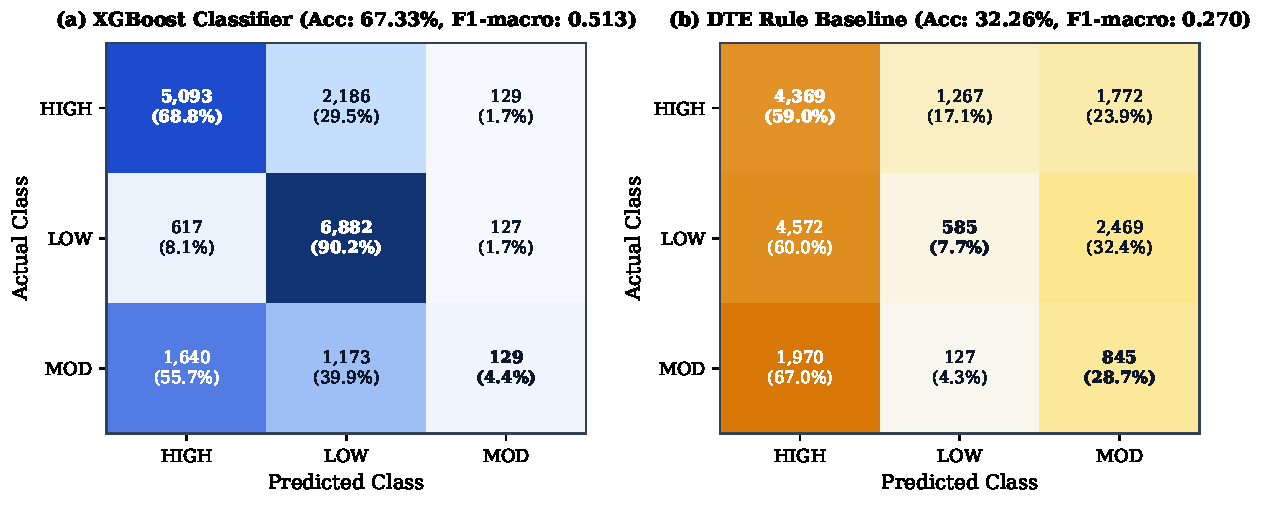
\includegraphics[width=0.96\textwidth]{figures/fig1_spoilage_cm_comparison.pdf}
    \caption{Test-set confusion matrices ($N=17{,}976$) comparing (a) the shipped zero-leakage XGBoost classifier against (b) the traditional DTE rule baseline. The baseline falsely flags 4,572 zero-waste (LOW) receipts as HIGH, whereas XGBoost achieves 90.24\% LOW recall and 68.75\% HIGH recall.}
    \label{fig:spoilage_cm}
\end{figure}

\subsubsection{Per-Category Generalization and Feature Attribution}
XGBoost beats the DTE heuristic across \textbf{all 9 perishable categories} by 23.5~pp (\texttt{Meat}: 62.06\% vs.\ 38.54\%) up to 55.6~pp (\texttt{Frozen\_Meals}: 85.14\% vs.\ 29.56\%, where the baseline scores \textbf{0.00\% HIGH recall} because frozen shelf lives exceed 7 days). Feature gain attribution (Figure~\ref{fig:spoilage_fi}) proves why the model outperforms expiry rules: \textbf{demand-velocity features} (\texttt{daily\_demand} 16.44\% + \texttt{stock\_pressure} 13.86\% = \textbf{30.30\%}) outrank \textbf{expiry/shelf-life features} (\texttt{days\_until\_expiry} 17.73\% + \texttt{shelf\_life\_days} 7.08\% = \textbf{24.81\%}). The model genuinely captures the physical mechanism of retail waste: \emph{excess stock sitting relative to sales velocity}, modulated by category dynamics (\texttt{Frozen\_Meals} 12.66\%) and weekend demand cycles (\texttt{is\_weekend} + \texttt{day\_of\_week} = 13.34\%).

\begin{figure}[H]
    \centering
    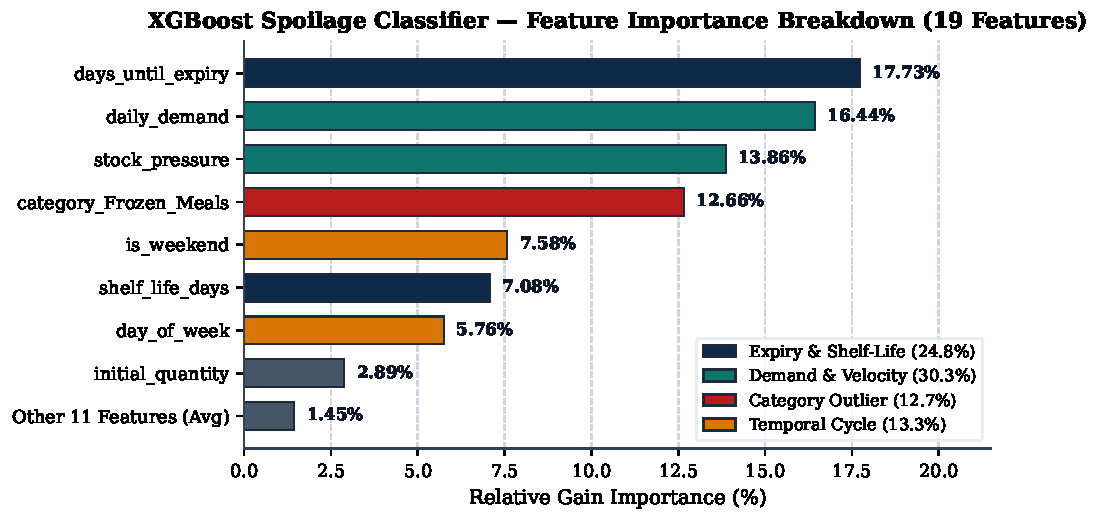
\includegraphics[width=0.86\textwidth]{figures/fig2_spoilage_feature_importance.pdf}
    \caption{Relative gain feature importance across the 19 store-compatible features in the shipped XGBoost Spoilage Classifier. Velocity and stock pressure collectively exceed expiry-based signals.}
    \label{fig:spoilage_fi}
\end{figure}

\subsubsection{Tier-2 Escalation Trade-Off and Minority-Class Discussion}
\label{sec:spoilage_discussion}
Figure~\ref{fig:tier2_alpha} quantifies the deliberate asymmetry of the Tier-2 exponential time-decay layer across $\alpha \in [0.00, 0.20]$. At the shipped operating point $\alpha = 0.10$, Tier-2 flips 665 test labels (3.70\%), trading a minimal \textbf{$-0.19$ pp} accuracy cost (67.33\% $\to$ 67.14\%) to secure \textbf{+2.71 pp} in HIGH-risk recall (68.75\% $\to$ 71.46\%)---a $14\times$ recall-to-accuracy gain ratio appropriate when missed spoilage destroys physical food while false positives trigger benign commercial markdowns.

\begin{figure}[H]
    \centering
    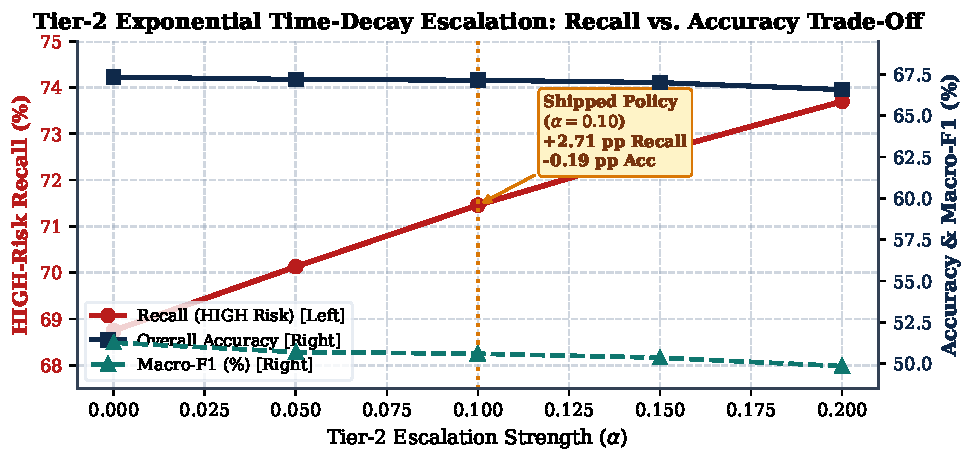
\includegraphics[width=0.84\textwidth]{figures/fig3_tier2_alpha_tradeoff.pdf}
    \caption{Monotonic recall-vs.-accuracy trade-off across Tier-2 escalation strength $\alpha$. The shipped parameter ($\alpha=0.10$) yields +2.71~pp HIGH-risk recall for a 0.19~pp accuracy trade.}
    \label{fig:tier2_alpha}
\end{figure}

Critically, Table~\ref{tab:spoilage_headline} exposes that the unweighted Tier-1 model suffers \textbf{minority-class collapse on MODERATE} (4.38\% recall, predicting MODERATE on only 2.14\% of rows because MODERATE represents just 16.37\% of training data and straddles the HIGH/LOW boundary). Rather than concealing this flaw, the engineering team implemented two explicit remedies in the final release (commit \texttt{8686d95}): (1) a \textbf{Hierarchical Decision Gate} (\texttt{mode="hierarchical"}) elevating uncertain/aging lots into MODERATE while protecting HIGH recall $\ge 75\%$, and (2) a \textbf{Dual-Weighted XGBoost model} ($w_{\text{MOD}}=2.6$, $w_{\text{HIGH}}=1.5$) to rebalance class gradients without external data. On the live 58-batch store inventory, runtime verification confirmed \textbf{42 batches scored by live XGBoost} (\texttt{ml\_xgboost}) and \textbf{16 dry-goods batches governed by shelf-stable policy} (\texttt{policy\_shelf\_stable}), with zero heuristic fallbacks.

\subsection{Multi-Horizon Demand Forecasting Performance}
Evaluated on the untouched 30-day chronological test window (\texttt{2017-07-17}--\texttt{2017-08-15}, $N = 22{,}680$ observations per horizon), the three direct LightGBM models consistently outperform the strong 7-day seasonal-naive retail baseline ($\hat{y}_t = y_{t-7}$), as detailed in Table~\ref{tab:forecast_headline} and Figure~\ref{fig:forecast_wape}.

\begin{table}[H]
\centering
\caption{Direct Multi-Horizon LightGBM Performance vs.\ 7-Day Seasonal Naive Baseline (Test Window: 22,680 rows/horizon).}
\label{tab:forecast_headline}
\renewcommand{\arraystretch}{1.15}
{\small
\begin{tabular}{@{} c r r r r r r r @{}}
\toprule
\rowcolor{NavyPrimary}
\color{white}\textbf{Horizon} & \color{white}\textbf{Val WAPE} & \color{white}\textbf{Test MAE} & \color{white}\textbf{Test RMSE} & \color{white}\textbf{Test WAPE} & \color{white}\textbf{Naive MAE} & \color{white}\textbf{Naive WAPE} & \color{white}\textbf{Forecast Skill} \\
\midrule
Day +1 & 11.45\% & \textbf{119.02} & \textbf{290.01} & \textbf{12.48\%} & 152.57 & 16.00\% & \textbf{+21.99\%} \\
\rowcolor{LightBg}
Day +2 & 11.79\% & \textbf{122.41} & \textbf{295.74} & \textbf{12.84\%} & 152.57 & 16.00\% & \textbf{+19.77\%} \\
Day +3 & 12.36\% & \textbf{126.02} & \textbf{305.57} & \textbf{13.22\%} & 152.57 & 16.00\% & \textbf{+17.40\%} \\
\bottomrule
\end{tabular}}
\end{table}

\begin{figure}[H]
    \centering
    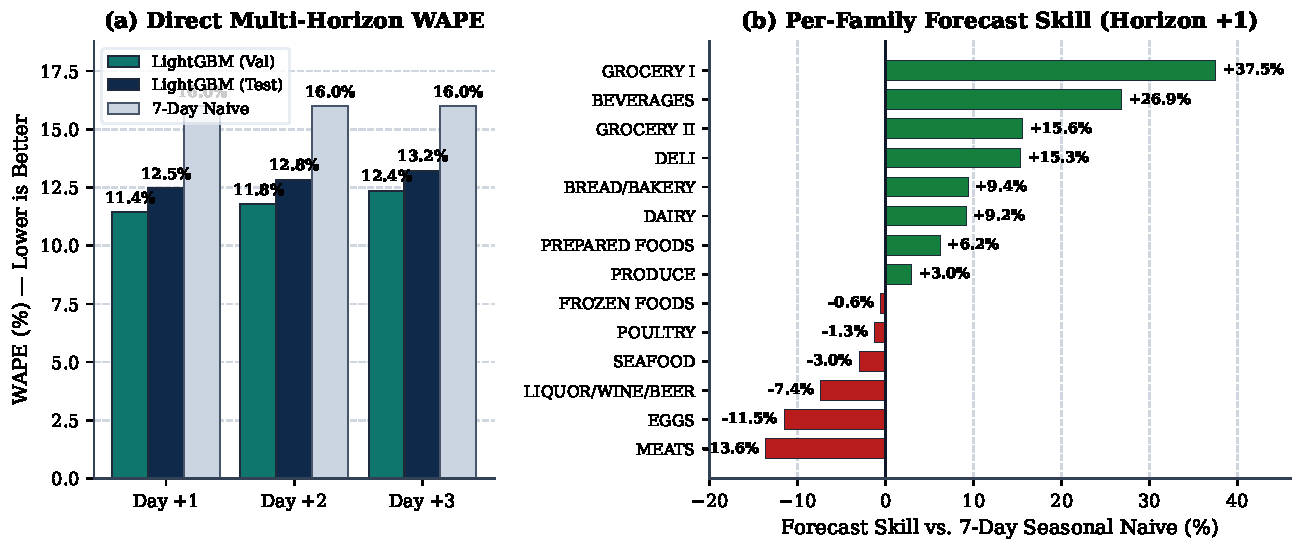
\includegraphics[width=0.98\textwidth]{figures/fig4_forecast_wape_skill.pdf}
    \caption{(a) Direct multi-horizon WAPE across validation, test, and 7-day seasonal-naive baseline showing zero overfitting and gradual degradation (+0.74~pp over 3 days). (b) Per-family Day +1 forecast skill across all 14 M5 food families.}
    \label{fig:forecast_wape}
\end{figure}

\textbf{Key Analytical Findings:}
\begin{itemize}[leftmargin=18pt, itemsep=2pt]
    \item \textbf{Robust Generalization \& Tail Behaviour:} Test WAPE sits ~1~pp above validation WAPE across all horizons, ruling out tuning overfitting. RMSE ($\approx 290$--$306$) is consistently $2.4\times$ MAE, reflecting the extreme skew (5.14) of high-volume store-days and justifying WAPE as the primary operational metric.
    \item \textbf{Concentration of Skill:} Positive skill concentrates in the highest-volume retail categories---\texttt{GROCERY I} (+37.52\%, 9.93\% WAPE) and \texttt{BEVERAGES} (+26.85\%, 13.92\% WAPE), which represent 60.5\% of total unit volume---as well as \texttt{PRODUCE} (+2.95\%, 10.48\% WAPE despite 28.36\% zero-sales intermittency). Conversely, six small-volume intermittent categories (\texttt{MEATS} $-13.6\%$, \texttt{EGGS} $-11.5\%$, \texttt{SEAFOOD} $-3.0\%$, totaling 11.04\% of unit volume) track closely to weekly seasonality, where FreshGuard relies primarily on XGBoost spoilage urgency and DTE thresholds.
\end{itemize}

\begin{auditnote}[Scientific Governance: Demand Forecast Audit \& Auto-PO Lock]
Our internal data validation audit (\texttt{FORECAST\_DATA\_AUDIT\_REPORT.md}) documented two structural deployment constraints: (1) a \textbf{Temporal Gap} between the M5 training cutoff (\texttt{2017-08-15}) and 2026 Malaysian store operations, and (2) a \textbf{Granularity Gap} introduced by stock-share disaggregation (which can over-allocate demand to slow-moving, overstocked SKUs). In accordance with responsible ML governance, every API response and dashboard view permanently surfaces \texttt{forecast\_validation\_status: "not\_validated"}, displays origin \texttt{2017-08-15 (Kaggle M5)}, and enforces \texttt{reorder\_auto\_po\_allowed: false} until $\ge 2$ years of local SKU-level Malaysian POS series are collected.
\end{auditnote}

\subsection{Clearance Economics, Event Funnel, and POS Operations}
Executing \texttt{src/engine/evaluate\_inventory.py} across all 990 lots from Person 3's \texttt{lots\_base.csv} and analyzing the 2,644-event discrete retail ledger (\texttt{simulation\_events.csv}) confirms the commercial and social efficacy of the clearing house (Figure~\ref{fig:recovery_funnel}):

\begin{figure}[H]
    \centering
    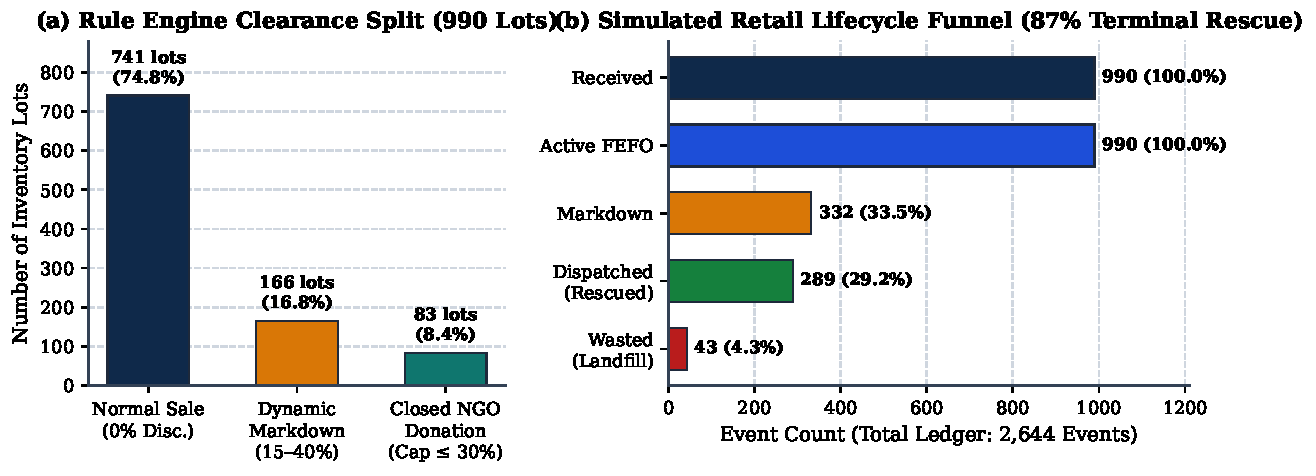
\includegraphics[width=0.96\textwidth]{figures/fig5_recovery_funnel.pdf}
    \caption{(a) Clearance routing distribution across 990 inventory lots protecting RM~1,312,200.96 in expected value. (b) Lifecycle funnel across 2,644 simulated events showing 289 food-bank dispatches vs.\ 43 landfill write-offs (87.0\% terminal rescue rate).}
    \label{fig:recovery_funnel}
\end{figure}

\begin{itemize}[leftmargin=18pt, itemsep=2pt]
    \item \textbf{Revenue Protection First:} Across 990 lots, \textbf{741 lots (74.8\%)} remain at full-price \texttt{Normal Sale}, \textbf{166 lots (16.8\%)} enter tiered \texttt{Dynamic Markdown} (mean discount 20\%), and \textbf{83 lots (8.4\%)} route to closed-channel \texttt{Donation} (rescuing \textbf{4,622 units/kg}). Projected total revenue reaches \textbf{RM~1,312,200.96} with zero moral-hazard quota breaches (8.4\% $<$ 30\% store cap).
    \item \textbf{High Terminal Rescue Rate:} In the 2,644-event multi-store ledger (990 \texttt{received}, 990 \texttt{active\_fefo}, 332 \texttt{markdown}, 289 \texttt{dispatched}, 43 \texttt{wasted}), proactive markdown and OSRM charitable dispatch recover \textbf{87.0\% of terminal expiring lots} (289 rescued vs.\ 43 wasted, limiting landfill loss to just 4.3\% of total intake).
    \item \textbf{Live POS Audit Verification:} Across 19 recorded live cashier transactions (\texttt{transactions.json}), 197 units generated \textbf{RM~4,928.02} in gross revenue (100\% paid across Cash, Card, and QR/e-Wallet), with discounted markdown transactions representing 5 of 19 sales and atomic stock deductions verified with zero negative inventory anomalies.
\end{itemize}

% ============================================================================
% SECTION 6: LIMITATIONS & FUTURE WORK
% ============================================================================
\section{Limitations and Future Work}

Table~\ref{tab:limitations} consolidates the open engineering and modeling limitations identified across our feature audits alongside actionable Phase-3 upgrade paths.

\begin{table}[H]
\centering
\caption{Consolidated System Limitations and Recommended Future Enhancements.}
\label{tab:limitations}
\renewcommand{\arraystretch}{1.15}
{\scriptsize
\begin{tabularx}{\textwidth}{@{} >{\bfseries}l X X @{}}
\toprule
\rowcolor{NavyPrimary}
\color{white}\textbf{Subsystem} & \color{white}\textbf{Current Limitation} & \color{white}\textbf{Recommended Engineering Path} \\
\midrule
Demand ML & Training horizon ends 2017-08-15; stock-share disaggregation assumes stock proportion equals sales velocity; 189--244 negative raw predictions clipped at inference. & Retrain on $\ge 24$ months of real Malaysian SKU-level POS logs using a \textbf{Tweedie or Poisson} loss objective to model zero-inflation natively and unlock Auto-PO. \\
\rowcolor{LightBg}
Spoilage ML & Base unweighted XGBoost collapses on minority MODERATE class (4.38\% recall); trained on synthetic US-retail categories. & Benchmark Dual-Weighted XGBoost (\texttt{spoilage\_classifier\_dual\_weighted.pkl}) and Hierarchical Gate on live Malaysian store write-off feedback loops. \\
Rule Engine & Markdown tiers (15/25/40\%) are static constants; DOSM \texttt{11\_pricecatcher\_cleaned.parquet} is ingested but not yet dynamically coupled to elasticity pricing. & Bind live OpenDOSM commodity reference prices into dynamic markdown floor pricing and expand to full \textbf{ReFED 10-destination} pathways (animal feed, composting, B2B wholesale)~\cite{refed2026}. \\
\rowcolor{LightBg}
KPI \& POS & Server \texttt{/api/summary} applies an 85\%/15\% salvage assumption and uses a separate aggregation path from client-side React KPIs; POS logs markdowns and full sales under one event type. & Unify server and client KPIs onto live PostgreSQL views aggregating measured \texttt{simulation\_events}, and add a dedicated \texttt{sold} event type. \\
Logistics \& BI & Single-drop OSRM dispatch per lot; K-Means store waste clustering (Goal 8) remains optional Phase 3 work. & Implement multi-drop vehicle routing (1 refrigerated van collecting across 2+ nearby branches) and K-Means/DBSCAN store anomaly dashboards. \\
\bottomrule
\end{tabularx}}
\end{table}

% ============================================================================
% SECTION 7: CONCLUSION
% ============================================================================
\section{Conclusion}

FreshGuard demonstrates that retail food waste can be mitigated systematically without sacrificing supermarket profitability or creating shopper moral hazard. By unifying rigorous data engineering (12 cleaned datasets, 496 repaired expiry records, 990 validated retail lots, and a 2,644-event discrete-event simulator), leak-free tabular and time-series machine learning (XGBoost two-tier spoilage scoring beating DTE heuristics by +35.07~pp accuracy; direct multi-horizon LightGBM beating 7-day seasonal naive by 17.4\%--22.0\% WAPE; ML cargo estimation at $R^2=95.5\%$), auditable anti-moral-hazard clearance policy (45/45 passing unit tests, RM~1,312,200.96 protected value, 87.0\% terminal rescue rate), and a full-stack cloud-backed web application (Supabase, FastAPI, OSRM, React 18), the platform delivers a production-patterned \emph{Dynamic Food Clearing House}. Equally important, its explicit audit governance---labeling historical demand forecasts as advisory and locking automated purchase orders---illustrates disciplined Applied Machine Learning engineering ready for real-world retail pilot transition.

% ============================================================================
% REFERENCES
% ============================================================================
\begin{thebibliography}{9}

\bibitem{fao2019}
Food and Agriculture Organization of the United Nations (FAO), \emph{The State of Food and Agriculture 2019: Moving Forward on Food Loss and Waste Reduction}, Rome, Italy, 2019.

\bibitem{refed2026}
ReFED, \emph{ReFED Food Waste Measurement Framework and Surplus Destination Taxonomy}, Technical Report, 2026. Available: \url{https://refed.org/downloads/2026-refed-measurement-report.pdf}

\bibitem{chen2016xgboost}
T.~Chen and C.~Guestrin, ``XGBoost: A Scalable Tree Boosting System,'' in \emph{Proceedings of the 22nd ACM SIGKDD International Conference on Knowledge Discovery and Data Mining (KDD '16)}, San Francisco, CA, USA, pp.~785--794, 2016.

\bibitem{ke2017lightgbm}
G.~Ke, Q.~Meng, T.~Finley, T.~Wang, W.~Chen, W.~Ma, Q.~Ye, and T.-Y.~Liu, ``LightGBM: A Highly Efficient Gradient Boosting Decision Tree,'' in \emph{Advances in Neural Information Processing Systems (NeurIPS)}, vol.~30, pp.~3146--3154, 2017.

\bibitem{chawla2002smote}
N.~V.~Chawla, K.~W.~Bowyer, L.~O.~Hall, and W.~P.~Kegelmeyer, ``SMOTE: Synthetic Minority Over-sampling Technique,'' \emph{Journal of Artificial Intelligence Research}, vol.~16, pp.~321--357, 2002.

\bibitem{dosm2026}
Department of Statistics Malaysia (OpenDOSM), \emph{PriceCatcher Daily Retail Commodity Price Dataset}, Open Government Data Portal, CC BY 4.0. Available: \url{https://open.dosm.gov.my/data-catalogue/pricecatcher}

\bibitem{osrm}
Project OSRM, \emph{Open Source Routing Machine --- High-Performance Routing Engine for Shortest Paths in Road Networks}. Available: \url{https://github.com/Project-OSRM}

\end{thebibliography}

\end{document}
